\documentclass{beamer}

\usepackage[utf8]{inputenc}
\usepackage[russian]{babel}
\usepackage{hyperref}
\usepackage{graphicx}
\usepackage{listings}
\usepackage{ucs}

\lstset{
    extendedchars=\true,
    inputencoding=utf8x
}

\usetheme{Warsaw}
\usecolortheme{lily}
\useoutertheme[subsection=false]{smoothbars}
\useinnertheme{circles}
\setbeamertemplate{footline}[page number]{}
\setbeamertemplate{navigation symbols}{}

\renewcommand{\figurename}{} 

\title{Архитектура ЭВМ}
\subtitle{Лекция 3. Что такое x86?}
\author{к.ф.-м.н. Филонов Павел Владимирович \\ filonovpv@gmail.com}
\date{15 сентября 2013 г.}


\institute[МГТУ ГА] 
{
    Московский Государственный Технический Университет \\
    Гражданской Авиации
}
\begin{document}
    \frame{\titlepage}
    \section{История Intel}
    \subsection{}
    \begin{frame}{Повестка дня}
    	\begin{enumerate}
    	\pause
    	\item Краткая история процессоров Intel
    	\pause
    	\item Архитектура x86
    	\pause
    	\item Что означают следующие надписи: x86-64, i386, IA-32, IA-64?
    	\pause
    	\item Кто пишет понятней: AT\&T или Intel?
    	\pause
    	\item NASM --- наше всё!
    	\pause
    	\item Макросы нам помогут!
    	\end{enumerate}
    \end{frame}
    \begin{frame}{Intel 4004 --- 1971 год}
    \begin{columns}
    	\column{0.4\linewidth}
    	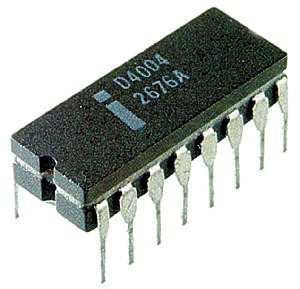
\includegraphics[width=0.7\linewidth]{fig/Intel_4004.jpg}
    	\footnotesize

    	Основные характеристики:
    	\begin{itemize}
    		\item Тактовая частота 92,6 кГц
    		\item Гарвардская архитектура
    		\item Объём адресуемой памяти: 640 байт
    		\item 16 4-х битных регистров
    		\item Число инструкций --- 46
    		\item Число транзисторов --- 2250 
    	\end{itemize}
    	\column{0.6\linewidth}
    	\begin{figure}
    		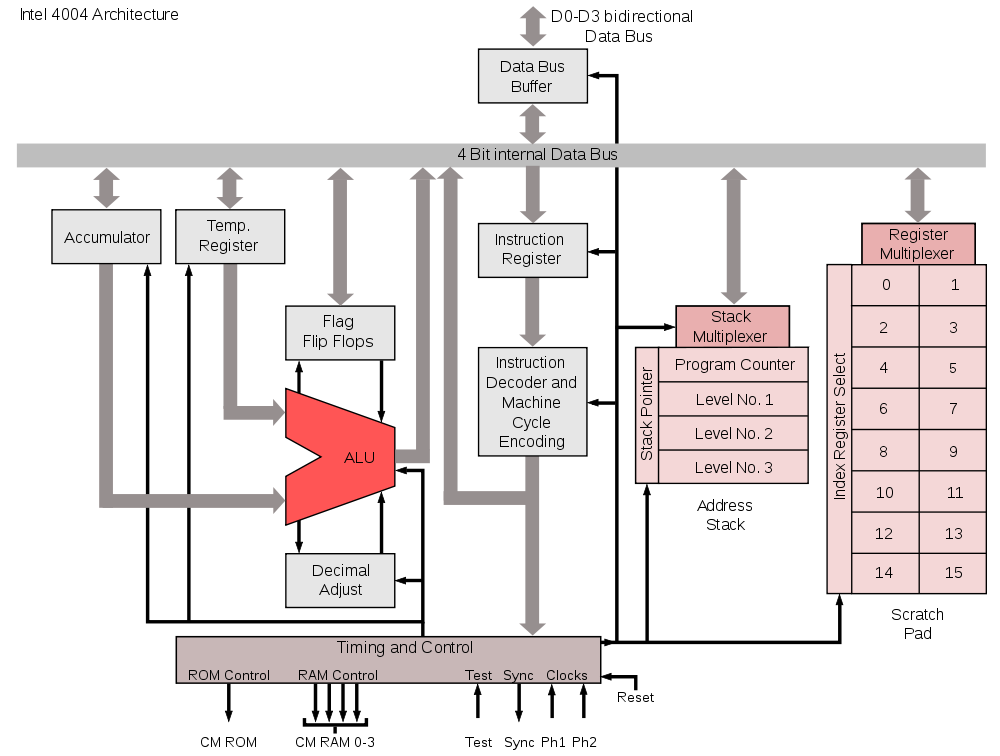
\includegraphics[width=\linewidth]{fig/4004_arch.png} \\
    		Блок-схема
    	\end{figure}
    \end{columns}
    \end{frame}
    \begin{frame}{Intel 8080 --- 1974 год}
    \begin{columns}
    	\column{0.4\linewidth}
    	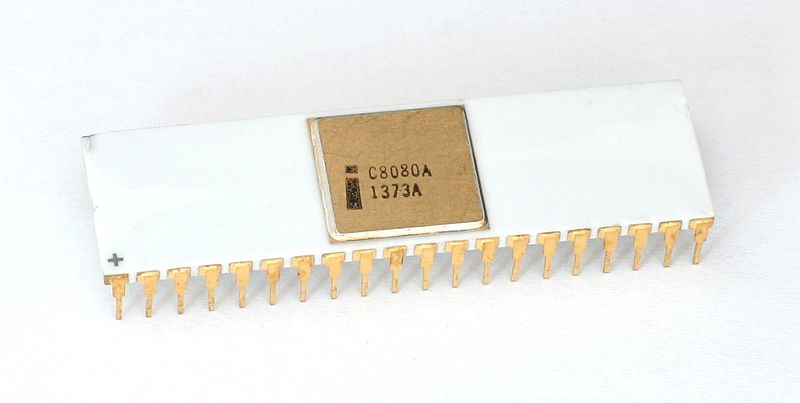
\includegraphics[width=0.8\linewidth]{fig/Intel_8080.jpg}
    	\footnotesize

    	Основные характеристики:
    	\begin{itemize}
    		\item Тактовая частота: 2 мГц
    		\item Прингстонская архитектура
    		\item Объём адресуемой памяти: 64 Кбайт
    		\item 7 8-ми битных регистров
    		\item Число инструкций --- 80
       		\item Число транзисторов --- 6000  
    	\end{itemize}
    	\column{0.6\linewidth}
    	\begin{figure}
    		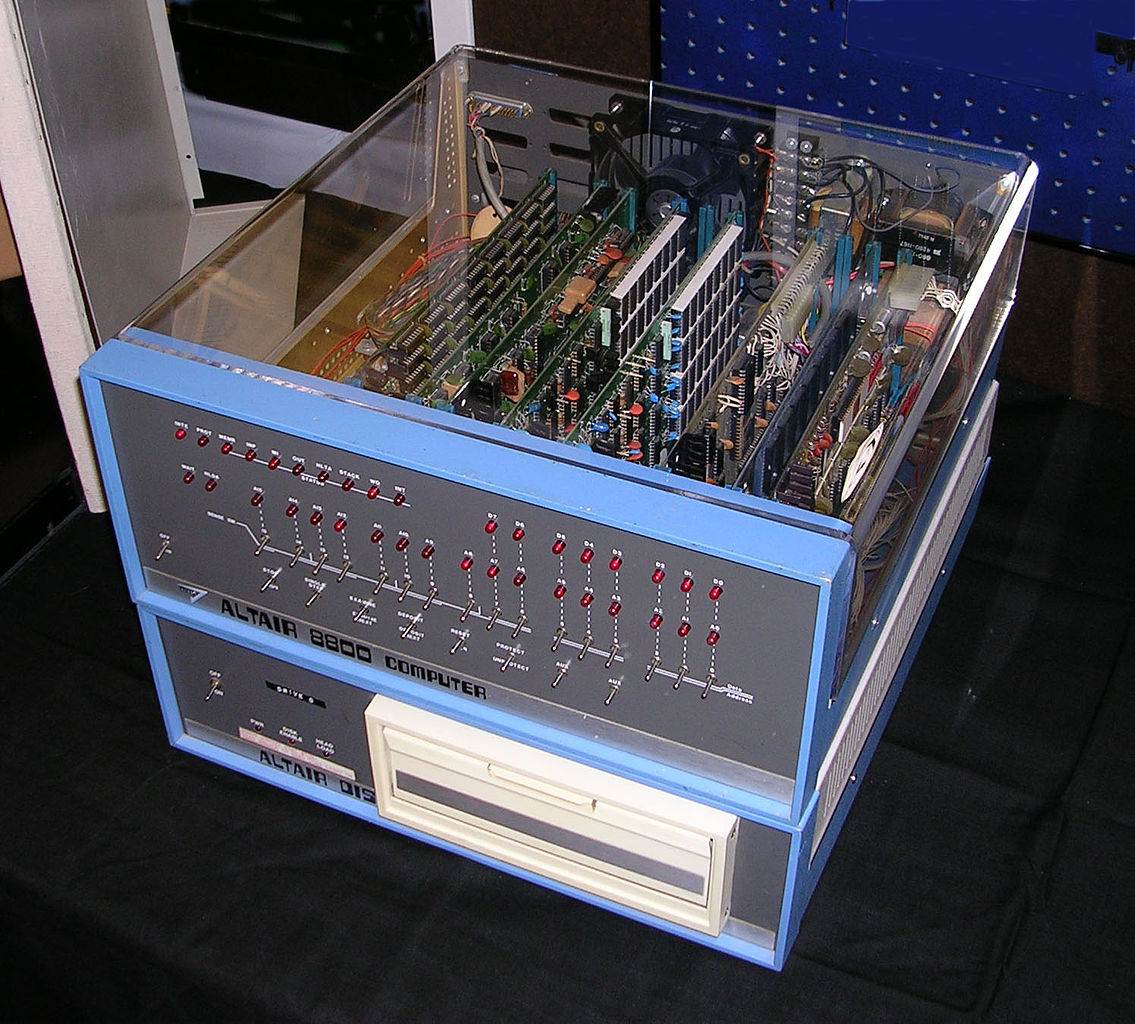
\includegraphics[width=\linewidth]{fig/Altair_8800.jpg}

    		Altair 8800
    	\end{figure}
    \end{columns}
    \end{frame}
    \begin{frame}{Intel 8088 --- 1979 год}
    \begin{columns}
    	\column{0.4\linewidth}
    	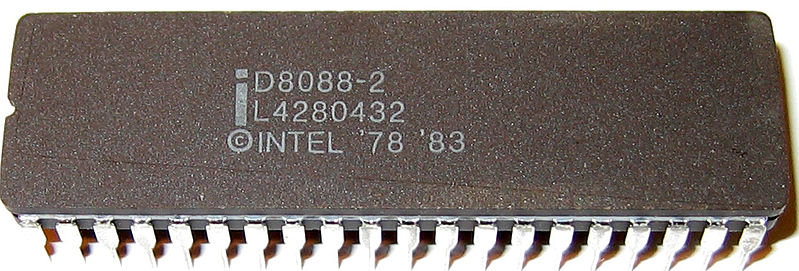
\includegraphics[width=0.8\linewidth]{fig/Intel_8088.jpg}
    	\footnotesize

    	Основные характеристики:
    	\begin{itemize}
    		\item Тактовая частота: 5 мГц
    		\item Объём адресуемой памяти: 1 Мбайт
    		\item 8 16-ти битных регистров
    		\item Число инструкций --- 98
    		\item Число транзисторов --- 29000  
    	\end{itemize}
    	\column{0.6\linewidth}
    	\begin{figure}
    		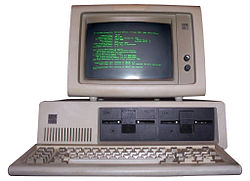
\includegraphics[width=\linewidth]{fig/IBM_PC.jpg}

    		IBM PC
    	\end{figure}
    \end{columns}
    \end{frame}
    \begin{frame}{Intel 80386 (i386) --- 1985 год}
    \begin{columns}
    	\column{0.4\linewidth}
    	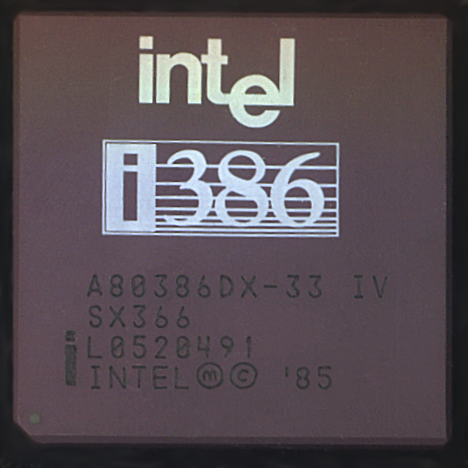
\includegraphics[width=0.7\linewidth]{fig/i386.png}
    	\footnotesize

    	Основные характеристики:
    	\begin{itemize}
    		\item Тактовая частота: 16, 20,25,33,40 мГц
    		\item Объём адресуемой памяти: 4 Гбайт
    		\item 8 32-х битных регистров
    		\item Число инструкций --- 150 (x86 или IA-32)
    		\item Число транзисторов --- 275000
    	\end{itemize}
    	\column{0.6\linewidth}
    		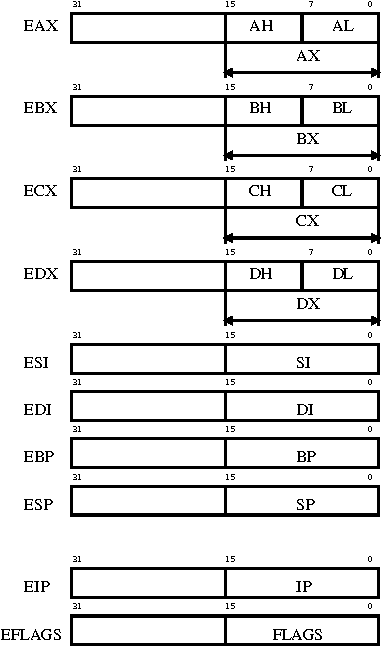
\includegraphics[width=0.7\linewidth]{fig/x86_regs.pdf}

    \end{columns}
    \end{frame}
    \begin{frame}{И остальные модели}
    	\begin{itemize}
    		\item {\bf i486} --- математический сопроцессор (FPU), кеш L1, L2
    		\item {\bf Pentium} --- суперскалярная архитектура, предсказание ветвлений, раздельное кеширование кода и данных
    		\item {\bf Pentium II} --- SIMD MMX инструкции
    		\item {\bf Pentium III} --- RISC-ядро, SSE (Streaming SIMD Extensions)
    		\item {\bf Pentium 4} --- Hyper-threading, SSE2, SSE3, EMT64T(x86-64 или IA-64)
    		\item {\bf Pentium D} --- 2 ядра
    		\item {\bf Core 2} --- 1,2,4 ядра, VT-x, SSSE3
    		\item {\bf Core i3,i5,i7} --- Hyper-threading, встроенный графический процессор, SSE4

    	\end{itemize}
    \end{frame}
    \section{x86}
    \subsection{}
    \begin{frame}{Архитектура x86}
        \begin{columns}
        \column{0.4\linewidth}
            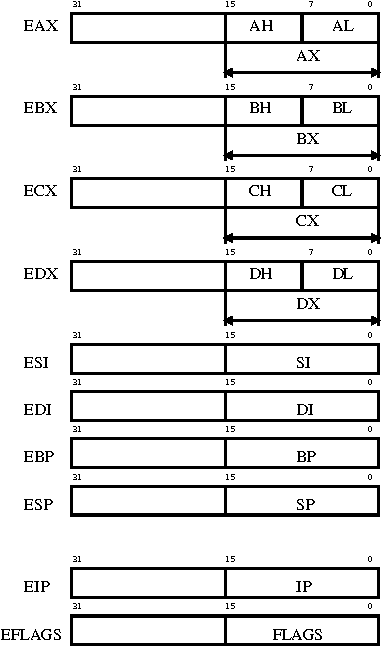
\includegraphics[width=\linewidth]{fig/x86_regs.pdf}
        \column{0.6\linewidth}
        \begin{itemize}\footnotesize
            \item Разрядность регистров --- 32 бита
            \begin{itemize}
                \item {\bf EAX} --- аккумулятор
                \item {\bf EBX} --- адрес данных
                \item {\bf ECX} --- счётчик циклов
                \item {\bf EDX} --- для хранения данных
                \item {\bf ESI} --- адрес источника
                \item {\bf EDI} --- адрес приёмника
                \item {\bf EBP} --- указатель на данные в стеке
                \item {\bf ESP} --- указатель на вершину стека
                \item {\bf EIP} --- счётчик команд
                \item {\bf EFLAGS} --- регистр флагов
            \end{itemize}
            \item Объём адресуемой памяти --- 4 Гбайта ($2^{32}$ байт)
            \item Плоская модель памяти
            \item Число инструкций общего назначения $\sim 257$
        \end{itemize}
        \end{columns}
    \end{frame}
    \begin{frame}{Регистр флагов EFLAGS}
    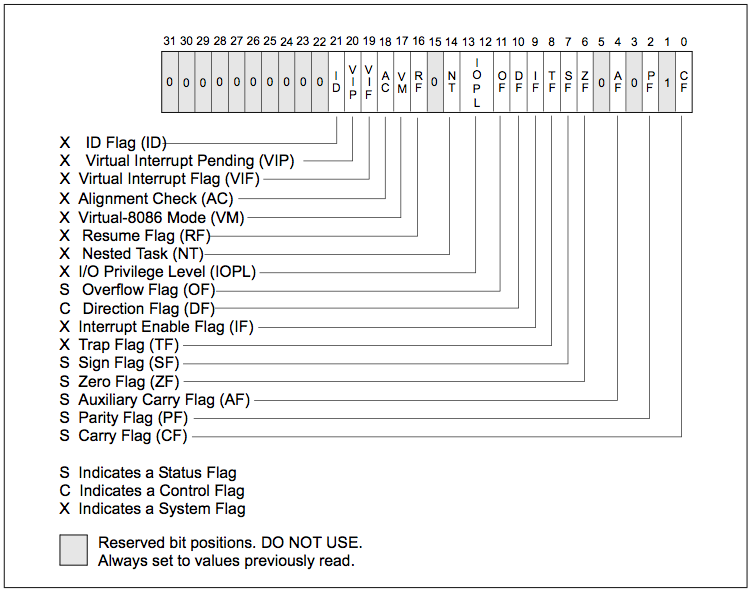
\includegraphics[width=0.9\linewidth]{fig/EFLAGS.png}
    \end{frame}
    \begin{frame}{Флаги состояния}
        \begin{itemize}
            \item {\bf ZF} --- zero flag (флаг нуля) показывает равенство результата нулю
            \item {\bf CF} --- carry flag (флаг переноса) показывает наличие переполнения в беззнаковой целочисленной арифметике
            \item {\bf SF} --- sign flags (флаг знака) показывает знак результата
            \item {\bf OF} --- overflow flags (флаг переполнения) показывает наличие переполнения в знаковой целочисленной арифметике
            \item {\bf PF} --- parity flags (флаг чётности)  показывает чётность результата
            \item {\bf AF} --- auxiliary carry flags (вспомогательный флаг переноса) показывает наличие переполнения а двоично-десятичной арифметике (binary coded deciaml, BCD)
            \item {\bf DF} --- direction flag (флаг направления)
        \end{itemize}
    \end{frame}
    \begin{frame}{Архитектура x86-64 (IA-64)}
        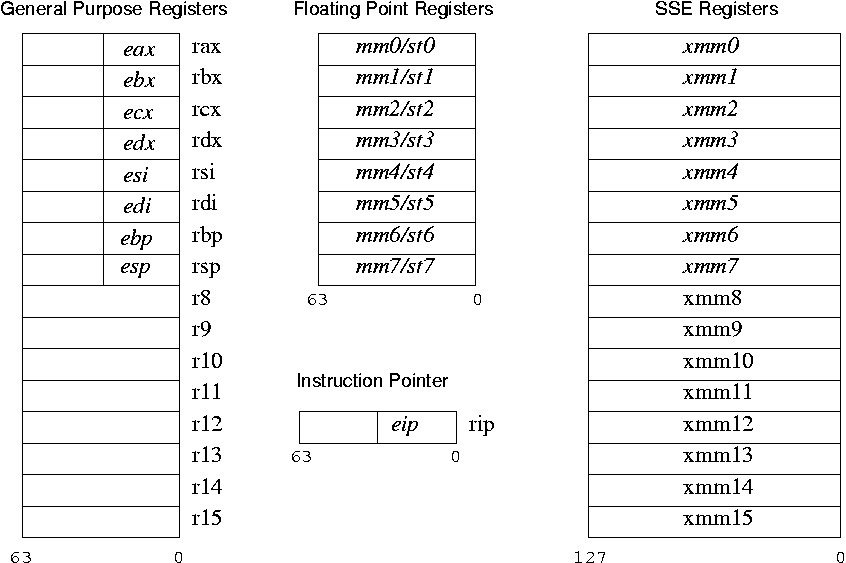
\includegraphics[width=\linewidth]{fig/x86-64.png}
    \end{frame}
    \begin{frame}{А какие ещё есть архитектуры процессоров?}
        \begin{itemize}
            \item ARM --- посмотрите на ваш мобильный телефон или планшет
            \item Atmel --- внимательно присмотритесь к стиральной машинке или холодильнику, а также поиграйтей с Arduino
            \item Microship PIC --- таже бытовая техника
            \item PowerPC --- до 2006 года основной процессор фирмы Apple
            \item SPARC --- замечательные числодробилки
            \item MIPS --- Sony PlayStation 2
        \end{itemize}
    \end{frame}
    \begin{frame}[fragile]
        \frametitle{Синтаксис ассемблера AT\&T и Intel для архитектуры x86}
        \begin{columns}
            \column{0.5\linewidth}
            \begin{block}{Intel}\footnotesize
            \begin{verbatim}
global _start 

section .data
    msg db 'Hello, world', 0x0A

section .text
_start:
    mov eax, 4
    mov ebx, 1
    mov ecx, msg
    mov edx, 13
    int 0x80
    
    mov eax, 1
    mov ebx, 0
    int 0x80
            \end{verbatim}
            \end{block}
            \column{0.5\linewidth}
            \begin{block}{AT\&T}\footnotesize
            \begin{verbatim}
.globl _start

.data
msg: .string "Hello, world\n"

.text
_start:
    movl $4,   %eax
    movl $1,   %ebx
    movl $msg, %ecx
    movl $13,  %edx
    int $0x80

    movl $1, %eax
    movl $0, %ebx
    int $0x80
            \end{verbatim}
            \end{block}
        \end{columns}    
\end{frame}
    \section{NASM}
    \subsection{}
    \begin{frame}{NASM --- Netwide Assembler (http://nasm.us)}
    Конкуренты: GAS, MASM, TASM, FASM, YASM
        \begin{block}{Преимущества}
            \begin{itemize}
                \item Использует Intel синтаксис (GAS уходит)
                \item Поддерживает как x86, так и x86-64 (TASM уходит)
                \item Поддерживает различные расширения (MMX, SSE*)
                \item Работает в различных ОС (Windows, DOS, Linux, FreeBSD, Mac OS X и др) (MASM уходит)
                \item Продолжает развиваться (Последняя версия YASM --- 2011 год)
                \item Есть литература на русском (FASM уходит) 
            \end{itemize}
        \end{block}
    \end{frame}
    \begin{frame}[fragile]
        \frametitle{Hello, world}
        \begin{block}{hello.asm}
        \begin{verbatim}
%include "stud_io.inc" ; подключаем файл с макросами
global _start   ; объявляет метку _start как глобальную

section .text   ; секция машинных команд
_start:         ; с метки _start начинается выполнение
  mov eax, 0    ; eax - счётчик цикла
again:          ; тело цикла
  PRINT "Hello" ; макрос вывода строк
  PUTCHAR 10    ; 10 - код символа переноса строки
  inc eax       ; eax := eax + 1
  cmp eax, 5    ; стравнить eax и 5 (eax - 5)
  jl again      ; jump less (прыгнуть если меньше)

  FINISH        ; макрос завершения программы
        \end{verbatim}
        \end{block}
\end{frame}
    \begin{frame}[fragile]
        \frametitle{Этапы сборки компилируемых программ}
        \begin{block}{Сборка и выполнение hello.asm}
        \begin{verbatim}
nasm -f elf -l hello.lst -o hello.o hello.asm
ld -o hello hello.o
./hello
        \end{verbatim}
        \end{block}
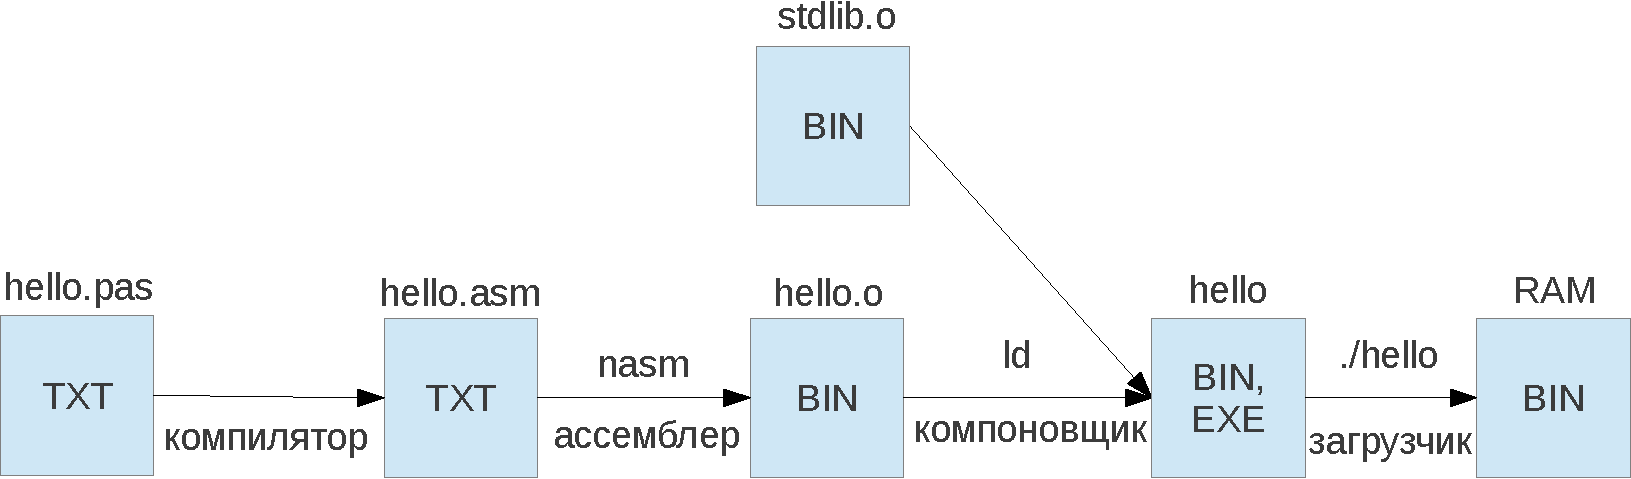
\includegraphics[width=\linewidth]{fig/build.pdf}
\end{frame}
    \begin{frame}{Макросы}

    {\bf Макрос} --- символьное имя, заменяющее несколько команд языка ассемблера

    \begin{block}{Макросы из stud\_io.inc}
        \begin{itemize}
            \item {\tt PRINT} --- принимает в качестве параметра текстовыую строку, окружённую кавычками или апострофами и выводит её на экран
            \item {\tt PUTCHAR} --- в качестве парметра принимает код символа, однобайтовый регистр ({\tt AL, AH, BL, BH, CL, CH, DL, DH}) или исполнительный адрес и выводит на экран символ с соответствующим кодом
            \item {\tt GETCHAR} --- считывает код символа с клавиатуры и сохраняет его код в регистре {\tt EAX}. Если символов больше нет, то в регистр {\tt EAX} записывается -1 (0xFFFFFFFF)
            \item {\tt FINISH} --- завершает выполнение программы
        \end{itemize}
    \end{block}
    \end{frame}
    \begin{frame}
    \begin{block}{Укажите правильную последовательность операций}
        \begin{enumerate}
            \item компоновка
            \item компиляция
            \item ассемблирование
            \item загрузка
            \item выполнение
        \end{enumerate}
        \pause
        Ответ: 2, 3, 1, 4, 5
    \end{block}
    \pause
    \begin{block}{Какая инструкция уменьшает значение регистра на 1?}
        \begin{enumerate}
            \item mov
            \item inc
            \item \alt<4>{{\color{green}dec}}{dec}
            \item cmp
        \end{enumerate}
    \end{block}
    \end{frame}
    \begin{frame}[fragile]
        \frametitle{Вопросы}
        \begin{block}{Что делает эта программа?}
        \begin{verbatim}
%include "stud_io.inc"
global _start

section .text
_start:
    mov eax, 10
again:
    PUTCHAR al
    dec eax
    cmp eax, 0
    jg again

    FINISH
        \end{verbatim}
        \end{block}
\end{frame}
    \begin{frame}[fragile]
        \frametitle{Вопросы}
        \begin{block}{Что делает эта программа?}
        \begin{verbatim}
%include "stud_io.inc"
global _start

section .text
_start:
    mov ecx, 0
again:
    GETCHAR
    cmp eax, -1
    je exit
    inc ecx
    jmp again
    
exit:
    FINISH
        \end{verbatim}
        \end{block}
\end{frame}
    \begin{frame}{Краткие итоги}
        \begin{block}{Что мы узнали сегодня}
        \begin{itemize}
            \item послушали краткую историю процессоров Intel
            \item узнали что такое x86 и чем он отличается от x86-64
            \item познакомились с азами архитектуры x86
            \item выбрали ассемблер для дальнейшей работы
            \item научились читать простые программы
        \end{itemize}
        \end{block}
    \end{frame}
\end{document}